The plot view allows you to view numerical molecule data in form of
two- or three-dimensional scatterplots. Any numerical data that is
stored in the database can be displayed by linking them either to
one of the three spatial axes or to the color and size attributes
of a dot in the diagram.

%
\begin{figure}[!htb]
\begin{centering}
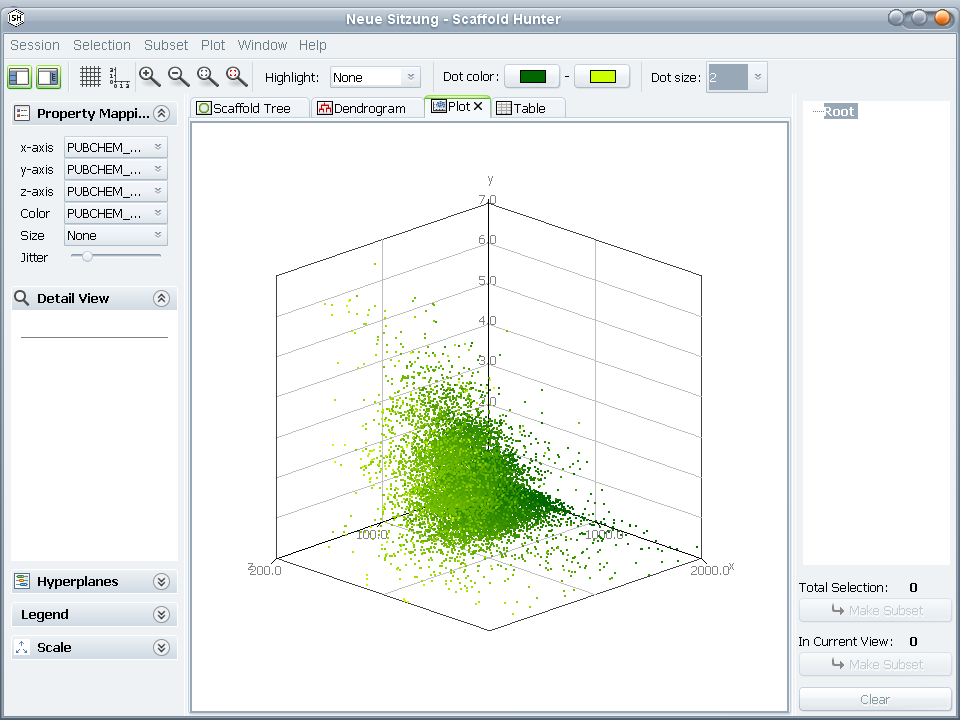
\includegraphics[width=0.8\columnwidth]{images/plot/plot_overview}
\par\end{centering}

\caption{The plot view}


%
\end{figure}



\subsection{Choosing the Data to be Displayed}

The first thing you want to do after opening a plot view is to select
the data that should be displayed. This can be done with the \textit{Property
Mapping} panel in the \sbar. Here you find a combo box for each of
the three spatial axes, for the dot color and the dot size, which allows
you to chose from numerical molecule properties. Additionally there is a slider
to apply a jitter to the data on the spatial axes.

%
\begin{figure}[!htb]
\begin{centering}
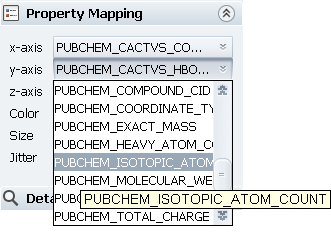
\includegraphics[width=0.3\columnwidth]{images/plot/property_mapping}
\par\end{centering}

\caption{The Property Mapping panel}
%
\end{figure}


Please note that the data has to be loaded from the database when
the mapping is changed. This can cause a slight delay before the diagram
is displayed. The mapping of data to axes is also shown in the \textit{Legend
panel} of the \sbar. There you can also see the domain of each
axis.


\subsection{Dot Color and Size}

The default color and size for dots can be changed at the \tbar.
These values are used when no data is mapped to the color/size properties.
As soon as you change the property mapping the elements in the \tbar
change to let you enter an interval for the color/size of the dots.

%
\begin{figure}
\begin{centering}
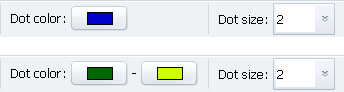
\includegraphics[width=0.3\columnwidth]{images/plot/dotcolor}
\par\end{centering}

\caption[Configuring dot colors]{The button for the color and the combo box for the dot size. The upper
figure shows the default behavior, when no data is mapped. The lower
figure shows the behavior when data is mapped to color/size.}
%
\end{figure}



\subsection{Hyperplanes}

Sometimes you do not want to see the complete set of data, but a small
part of it. This is where the concept of hyperplanes becomes useful.
Hyperplanes allow you to define thresholds for an axis, that means
a minimum and a maximum value that a data must have to be displayed
as dot in the diagram. They can be applied to any of the 5 dimensions (x,
y, z, color and size). When hyperplanes are set the associated threshold
values are shown in the diagram as black lines.

%
\begin{figure}[!htb]
\begin{centering}
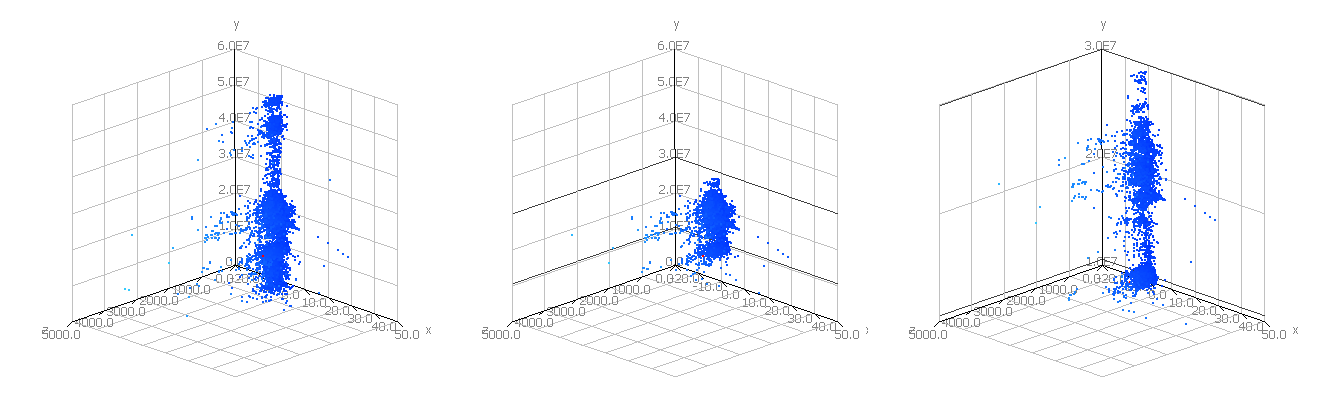
\includegraphics[width=1.0\columnwidth]{images/plot/hyperplane_example}
\par\end{centering}

\caption[Use of hyperplanes]{The use of hyperplanes in a diagram: Without hyperplanes (left figure),
with hyperplanes at the y-axis (middle) and with the y-axis adjusting
to the hyperplanes (right figure).}


%
\end{figure}


Hyperplanes can be set and adjusted using the Hyperplanes panel in
the \sbar. For each of the 5 possible dimensions there is a slider that
lets you change the upper and the lower threshold value. For a better
control the values can also be entered as numbers in the text fields. 

%
\begin{figure}[!htb]
\begin{centering}
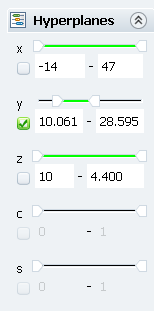
\includegraphics[width=0.18\columnwidth]{images/plot/hyperplane_panel}
\par\end{centering}

\caption{The hyperplane panel}
%
\end{figure}


While the axes always try to adjust themselves to the domain that
is mapped this behavior may be inappropriate when using hyperplanes.
By default a hyperplane does not influence the domain of an axis,
it just defines which values should be shown and which not. To let
an axis adjust according to the visible range that is defined by the
hyperplanes, click the checkbox for the axis in the panel.


\subsection{Zooming, Scrolling and Rotating the Diagram}

The diagram can be zoomed by using the buttons in the \tbar or by
using the mouse wheel. When using the mouse wheel the diagram will be
zoomed with keeping the focus at the current position of the mouse pointer.
Furthermore each axis can be scaled independently by using the buttons
in the Scale panel of the \sbar. In case the diagram becomes too
large to fit in the window you can scroll around by clicking in the
diagram with the left mouse button and drag it around. Rotating the
diagram works similar, just press the right mouse button while dragging.
Rotation only works in 3D-mode.

The \textit{Fit Graph} button in the \tbar always resets the zoom,
scroll position and rotation angles. Zooming and scrolling the diagram
to show the current selection can be done by clicking the button ``Zoom
to current selection'' in the \tbar.


\subsection{Highlighting, Selecting and Picking}

To avoid confusion with the dot colors the current selection and flags
(public and private) are not shown in the diagram by default. To make
them visible you have to set the accordant highlighting mode, which
can be done with the combo box in the \tbar. When the highlighting
mode is set to ``Selection'' then the dots that represent the
molecules in the current selection are shown in red. Setting the highlighting
mode to ``Public flag'' shows the molecules with a public flag
in green, while the highlighting mode ``Private flag'' shows the
molecules with a private flag in blue.

These features can also be set and removed from a molecule in the
plot view, according to Table~\ref{tableview mouse actions table}.

\begin{table}[!htb]
  \centering
  \begin{tabular}{p{0.3\columnwidth}p{0.55\columnwidth}}
  \textbf{Effect} & \textbf{Action}\\ \toprule
  add a molecule to or remove it from the selection & place the mouse pointer over the dot and click the left mouse button\\ \hline

  add multiple molecules to the selection & hold the \texttt{Shift} key and the left mouse button down while drawing a box
  around the dots\\ \hline

  remove multiple molecules from the selection & hold the \texttt{Ctrl} key and the left mouse button down while drawing a box
  around the dots\\ \hline

  toggle the public flag of a molecule & place the mouse pointer over the dot and click the middle mouse button\\ \hline

  toggle the private flag of a molecule & place the mouse pointer over the dot and click the middle mouse button
  while pressing the \texttt{Shift} key\\ \bottomrule
  \end{tabular}
  \caption{\Pview Mouse Actions}
  \label{tableview mouse actions table}
\end{table}



Please note that the highlighting mode adjusts automatically to the
action that is performed.

In any case, no matter if you perform one of these actions or not, the
molecule that belongs to the dot under the mouse pointer is shown in
the \textit{Detail View} panel in the \sbar.


\subsection{Hiding the Axis Ticks and Grids}

To toggle display of the axis ticks and grids there are two buttons
in the \tbar:
\begin{itemize}
\item 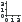
\includegraphics{images/plot/plot_toggle_ticks} this
button toggles the display of the ticks
\item 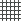
\includegraphics{images/plot/plot_toggle_grid}this
button toggles the display of the grids
\end{itemize}
